%D�finir le format du document: papier, taille de police, type de document, etc.
\documentclass[a4paper, 11pt]{article}

%%%%%%%%% Packages externes utilis�s %%%%%%%%%%%%%%%%%%%
\usepackage[french]{babel}
\usepackage[latin1]{inputenc}
\usepackage[T1]{fontenc}
\usepackage{verbatim}
\usepackage{graphicx}
\usepackage{epstopdf}
\usepackage{amsmath}
\usepackage{amssymb}
\usepackage{macro}
\usepackage{algorithm}
\usepackage{algorithmic}
%\usepackage{algorithm2e}


%La mise en page du rapport, NE PAS MODIFIER.
\usepackage{geometry}
 \geometry{
 a4paper,
 left=20mm,
 right=20mm,
 top=20mm,
 bottom=20mm,
 }

%%%%%%%%% Le corps du document entre begin et end %%%%%%%%%%%%%%%%%%%
\begin{document}

\section*{Video Stream}
\label{sec:Video_Stream}

\noindent Once connected to the GoPro camera, the drone can send a video stream to an other device.


\subsection*{Prerequisites}
\label{sec:Prerequisites}

\paragraph{Request} First of all to request the data stream, you have to connect to the WiFi network of the drone and you need to initialize a TCP connection to the controller in order that it know the host.


\subsection*{Protocol}
\label{sec:Protocol}

\paragraph{} 


\begin{figure}[H]
	\centering
		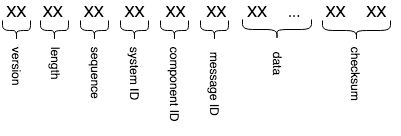
\includegraphics[scale=0.6]{./images/frame.png}
		\caption{The fields' names}
	\label{fig:frame}
\end{figure}

\paragraph{} 



\subsection*{Sources}
\label{sec:Sources}

\begin{itemize}
\item Streaming live video from the 3DR Solo : https://www.markturner.net/2017/02/06/streaming-live-video-from-the-3dr-solo/
\end{itemize}




\end{document}
